\documentclass[
	12pt,
	a4paper,
	oneside,
	english,
	brazil,
]{abntex2}

\usepackage{lmodern}
\usepackage{relsize}
\usepackage[T1]{fontenc}
\usepackage[utf8]{inputenc}
\usepackage{mathtools}
\usepackage{amssymb}

\newcommand{\beq}[1]{\mathlarger{#1}}

\titulo{Anotações de Estatística}
\autor{\(\alpha\)}
\local{Salvador}
\data{2020}

% informacoes do PDF
\makeatletter
\hypersetup{
     	%pagebackref=true,
		pdftitle={\@title}, 
		pdfauthor={\@author},
    		pdfsubject={\imprimirpreambulo},
	    	pdfcreator={LaTeX with abnTeX2},
		pdfkeywords={abnt}{latex}{abntex}{abntex2}{trabalho acadêmico}, 
		bookmarksdepth=4
}
\makeatother
% --- 

\setlength{\parindent}{0.6cm}
\setlength{\parskip}{0.2cm}
\makeindex

\begin{document}

\selectlanguage{brazil}
\frenchspacing 

\pretextual
\imprimircapa

% Epígrafe
\begin{epigrafe}
    \vspace*{\fill}
	\begin{flushright}
		\textit{Este resumo é inteiramente baseado no material de aula da Prof\textsuperscript{a} Julienne Borges da PUC Minas. Ele não pode e não deve ser publicado, muito menos utilizado para fins comerciais. Trata-se de um compilado dos assuntos da disciplina de Estatística da Pós-Graduação em Inteligência Artificial e Aprendizado de Máquina da referida universidade.}
	\end{flushright}
\end{epigrafe}
% ---

% Sumario
\pdfbookmark[0]{\contentsname}{toc}
\tableofcontents*
\cleardoublepage

\textual
\chapter{Introdução}

A estatística envolve técnicas para coletar, organizar,
descrever, analisar e interpretar dados provenientes de
experimentos ou vindos de outros estudos
observacionais.

\section{Conceitos básicos}

\begin{itemize}
	\item População: conjunto de todos os resultados, respostas, medidas ou contagens a serem estudados;
	\item Censo: conjunto de dados relativos a todos os elementos de uma população;
	\item Dados: informações provenientes de observações, contagens, medidas ou respostas;
	\item Amostra: subconjunto de elementos de uma população;
	\item Amostragem: processo de seleção da amostra.
	\item Parâmetro: medida que descreve numericamente uma característica da população.
	\item Estatística: medida que descreve numericamente uma característica da amostra.
\end{itemize}

\section{Tipos de Dados}

\begin{itemize}
	\item Qualitativos (ou categóricos): representam atributos, qualidades, características. Podem ser subdivididos em \textbf{nominais}(quando não possuem um ordem ou hierarquia) e \textbf{ordinais} (quando possuem uma ordem ou hierarquia);
	\item Quantitativos (ou não categóricos): consistem em medidas ou contagens. Podem ser subdivididos em \textbf{discretos} (conjunto finito ou enumerável de valores possíveis) ou \textbf{contínuos} (conjunto infinito de valores possíveis).
\end{itemize}
\chapter{Estatística Descritiva}

\section{Medidas de Tendência Central}

Mostram o valor em torno do qual os dados tendem a agrupar-se.

\subsection{Média Aritmética}

Notações:

\(\bar{x}\) Notação da média aritmática \emph{da amostra}

\(\mu\) Notação da média aritmática \emph{da população}

\[\bar{x} = \sum_{i=1}^{n} x_i \] 

\subsection{Mediana}

Notação: \(\tilde{x}\)

Seja \(n\) o tamanho da amostra:
\begin{itemize}
	\item O conjunto de dados da amostra precisa estar ordenado.
	\item Se \(n\) for ímpar, a mediana será o valor que ocupa a posição \(\frac{n + 1}{2}\)
	\item Se \(n\) for par, a mediana será a média dos valores que ocupam as posições \(\frac{n}{2}\) e \(\frac{n + 2}{2}\)
\end{itemize}

\section{Medidas de Posição Relativa}

Mostram pontos de corte na distribuição relativa dos dados da amostra.

\subsection{Percentil}

\[L = \frac{k}{100} \times n\]

Onde:

\(n\) = tamanho da amostra

\(k\) = percentil que se deseja calcular	

\(L\) = posição do percentil na amostra

\begin{itemize}
    \item Se \(L\) é um número inteiro, o percentil \(P_k\) pode ser obtido pela média 			entre os valores que ocupam as posições \(L\) e \(L+1\).
    \item Se \(L\) é um número decimal, devemos arredondar \(L\) para o valor interiro 			mais próximo \emph{a maior} e o percentil \(P_k\) será obtido pelo valor que ocupa a 		posição \(L\) já arredondada.      
\end{itemize}

\subsection{Escore z}

\[z = \frac{x-\bar{x}}{s}\]

\(z\) = \emph{escore z}

\(x\) = valor na amostra a partir do qual se quer medir o \emph{escore z}

\(\bar{x}\) = média aritmética da amostra

\(s\) = desvio padrão da amostra

\section{Medidas de Dispersão ou Variabilidade}

Mostram o grau de afastamento dos valores observados em relação ao ponto central da distribuição dos dados.

\subsection{Variância e Desvio Padrão}

\begin{table}[h]
	\centering	
	\caption{Notações de Variância e Desvio Padrão}
	\begin{tabular}{l|cc} 
		Medidas 		& População 	& Amostra 		\\
		\hline
		Variância		& \(\sigma^2 \)	& \(s^2\)	\\
		Desvio Padrão	& \(\sigma \)	& \(s\)
	\end{tabular}
\end{table}

Variância (população):

\[ \sigma^2=\frac{\sum_{i=1}^{n} (x_i - \bar{x})^2}{n} \]

Variância (amostra):

\[ s^2=\frac{\sum_{i=1}^{n} (x_i - \bar{x})^2}{n-1} \]

Desvio Padrão (população):

\[ \sigma=\sqrt{\frac{\sum_{i=1}^{n} (x_i - \bar{x})^2}{n}} \]

Desvio Padrão (amostra):

\[ s=\sqrt{\frac{\sum_{i=1}^{n} (x_i - \bar{x})^2}{n-1}} \]

\subsection{Coeficiente de Variação}

\[ CV=\frac{s}{\bar{x}} \times 100 \]
\chapter{Probabilidade}

Probabilidade é a teoria matemática utilizada para se estudar a incerteza oriunda de fenômenos de caráter aleatório. Fornece a base para os métodos que utilizamos quando fazemos generalizações a partir de dados observados.

A \textbf{Probabilidade} em si é uma médida numérica (variando de 0 a 1) da possibilidade de um evento ocorrer. Ela estuda situações onde os resultados são variáveis:
\begin{itemize}
	\item Os resultados possíveis são conhecidos;
	\item Não se pode saber \textit{a priori} qual deles ocorrerá.
\end{itemize}

\textbf{Experimentos Aleatórios} são aqueles cujos resultados podem não ser os mesmos, ainda que sejam repetidos sob condições idênticas:
\begin{itemize}
	\item O resultado de um experimento aleatório específico não é previamente conhecido;
	\item Todos os possíveis resultados podem ser descritos.
\end{itemize}

\textbf{Espaço Amostral} ( \(\Omega\) ) é o conjunto de todos os possíveis resultados de um experimento aleatório:
\begin{itemize}
	\item \(\Omega_1 = \{ 1, 2, 3, 4, 5, 6 \} \) - Faces de um dado
	\item \(\Omega_2 = \{ t \in R \mid t \geq 0 \} \) - Vida útil de uma lâmpada
\end{itemize}

\textbf{Evento} é um subconjunto do espaço amostral:
\begin{itemize}
	\item \(A_1 = \{ 2, 4, 6 \} \) - Obter uma face par do dado
	\item \(B_2 = \{ t \geq 10000 \} \) - A lâmpada durar pelo menos 10000 minutos
\end{itemize}

\section{Axiomas de Probabilidade}

Dado um espaço amostral, \(\Omega\), suponha que estamos estudando um evento A. A
probabilidade do evento A ocorrer é denotada por P(A). A função P(A) só será uma
probabilidade se ela satisfaz três condições básicas:
\begin{itemize}
	\item \( 0 \leq P(A) \leq 1 \)
	\item \( P(\Omega) = 1 \)
	\item \( P(A_1 \cup A_2 \cup A_3...) = P(A_1)+P(A_2)+P(A_3)+...\), se os eventos \(A_1, A_2, A_3, ...\) forem disjuntos (mutuamente exclusivos).
\end{itemize}

\section{Atribuição de Probabilidade aos Elementos de \( \Omega \)}

Visão Clássica:

\[ P(A) = \frac{casos favoráveis}{total de casos} \]

Visão Frequentista:

\[ P(A) = \frac{ocorrências de A}{repetições do experimento} \]

Interseção de Eventos: 

\[ A \cap B \]

Eventos Disjuntos: 

\[ A \cap B = \varnothing \]

União de 2 Eventos:

\[ P(A \cup B) = P(A) + P(B) - P(A \cap B) \]  

Eventos Complementares:

\[ A \cup B = \Omega \] 
\[ A \cap B = \varnothing \]
\[ \bar{A} = B \]
\[ \bar{B} = A \]
\[ P(A) = 1 - P(B) \]
\[ P(\bar{A}) = P(B) = 1 - P(A) \]

\subsection{Probabilidade Condicional}

Probabilidade de um evento A ocorrer dado que um evento B já ocorreu:

\[ P(A \mid B) = \frac{P(A \cap B)}{P(B)} \]

A partir da qual é possível deduzir a \textbf{regra do produto condicional}:

\[ P(A \cap B) = P(A \mid B).P(B) \]

Dois eventos podem ser considerados independentes quando \( P(A \mid B) = P(A) \) e \( P(B \mid A) = P(B) \). É possível deduzir também que, para A e B serem independentes, \( P(A \cap B) = P(A).P(B) \). 

\section{Variáveis Aleatórias}

O resultado de um experimento probabilístico pode ser frequentemente uma contagem ou uma medida. Quando isso ocorre, o resultado é chamado de variável aleatória. A variável aleatória \textbf{x} representa um valor numérico associado a cada um dos resultados de um experimento probabilístico.

\section{Modelos Probabilísticos para Variáveis Aleatórias Discretas}

Uma variável aleatória \textbf{X} é discreta se assume valores (x) que podem ser contados, ou seja, se houver um número finito ou contável de resultados possíveis que possam ser enumerados.

\subsection{Distribuição Binomial}

Condições:
\begin{itemize}
	\item n tentativas independentes
	\item X pode assumir os valores 0, 1, 2,..., n
	\item Probabilidade de sucesso em n tentivas = p
	\item Probabilidade de fracasso em n tentativas = q
	\item p + q = 1
\end{itemize}

Nestas condições, o comportamento de X pode ser descrito pela \textbf{Distribuição Binomial} com parâmetro n. 

\begin{itemize}
	\item Notação: \(X \sim B(n; p) \)
	\item Média de X: \( E(x) = n.p \)
	\item Variância de X: \( \sigma^2 = n.p.q \), onde q = 1 -p
\end{itemize}

Função de probabilidade de \(X \sim B(n; p) \):

\[\beq{ P(X = x) = \binom{n}{x} p^x (1 - p)^{n-x} }\]  

Onde \(\beq{ \binom{n}{x} }\) representa o coeficiente binomial calculado por \(\beq{ \binom{n}{x} = \frac{n!}{x!(n-x)!} }\) 

\subsection{Distribuição Poisson}

Condições:
\begin{itemize}
	\item a variável aleatória (X) consiste na contagem de eventos discretos que ocorrem em um meio contínuo (tempo, volume, área, etc.);
	\item \( \lambda \ > 0 \) é o número médio de eventos ocorrendo no intervalo considerado.
\end{itemize}

Nestas condições, o comportamento de X pode ser descrito pela \textbf{Distribuição de Poisson} com parâmetro 
\( \lambda \). 

\begin{itemize}
	\item Notação: \(X \sim Po( \lambda ) \)
	\item Média de X: \( E(X) = \lambda \)
	\item Variância de X: \( V(X) = \lambda \)
\end{itemize}

\section{Modelos Probabilísticos para Variáveis Aleatórias Contínuas}

Uma variável é considerada contínua quando pode assumir qualquer valor dentro de um intervalo, ou seja, se houver um número incontável de resultados possíveis, representados por um intervalo sobre o eixo real.

\subsection{Distribuição Polinomial}

\begin{itemize}
	\item Notação: \(X \sim Exp( \alpha ) \)
	\item Média de X: \( E(X) = \frac{1}{\alpha} \)
	\item Variância de X: \( V(X) = \frac{1}{\alpha^2} \)
\end{itemize}

Função de densidade de probabilidade (f.d.p.):

\[ f(x) =
  \begin{cases}
    \alpha e^{- \alpha x}    & \text{se } x>0 \text{ e } \alpha>0\\
    0 		& \text{ ,para quaisuqer outros valores}
  \end{cases}
\]

Probabilidade de X para um intervalo de \textbf{a} até \textbf{b}\footnote{Nesse cenário o fato de \textbf{a} e \textbf{b} estarem ou não no intervalo citado é irrelevante para o cálculo da probabilidade.}:

\[\beq{ P( a \leq X \leq b ) = e^{- \alpha a} - e^{- \alpha b} }\]


\subsection{Distribuição Normal}

Propriedades:
\begin{itemize}
	\item A distribuição é simétrica em torno da média, assim, as medidas de tendência central (média, mediana e moda) apresentam o mesmo valor;
 	\item A distribuição normal fica delimitada pelo seu desvio padrão e sua média. Cada combinação de valores de média e desvio padrão gera uma distribuição Normal diferente;
	\item A área sob a curva corresponde à 1;
	\item O ponto máximo da curva da distribuição normal ocorre quando x = \(\mu\), ou seja, em torno da média registra-se uma probabilidade maior de ocorrência. 
	\item À medida que nos afastamos da média, as probabilidades de ocorrência vão diminuindo.
\end{itemize}

Notação: \(X \sim N( \mu , \sigma^2 ) \)

Função de densidade de probabilidade (f.d.p.), para \( - \infty < x < \infty \):


\[\beq{ f(x) = \frac{1}{\sigma\sqrt{2\pi}} e^{\frac{-(x-\mu)^2}{2\sigma^2}{}} }\]

\subsubsection{Distribuição Normal Padrão}

O cálculo de probabilidades, para variáveis adequadamente descritas pela distribuição normal, é realizado por meio da distribuição normal padrão, também chamada de padronizada ou reduzida. A variável aleatória Z tem distribuição normal padrão, pois sua média é igual a zero e sua variância é igual a 1, ou seja, \( Z \sim N (0, 1) \).

Função de densidade de probabilidade (f.d.p.), para a Distribuição Normal Padrão (\( \mu = 0 \) e \( \sigma^2 = 1 \)):


\[\beq{ f(z) = \frac{1}{\sqrt{2\pi}} e^{\frac{-(z)^2}{2}{}} }\]

Redução do valor de uma variável aleatória X para a Distribuição Normal Padrão:

\[\beq{ z = \frac{x - \mu}{\sigma} }\]

\chapter{Inferência Estatística}

A estimação é o processo que consiste em utilizar dados amostrais para estimar os valores de parâmetros populacionais desconhecidos. 

\section{Estimativa Pontual}

A \textbf{estimativa é pontual} quando a estatística amostral origina uma única estimativa do parâmetro, ou seja, um único valor para o parâmetro populacional que se quer estimar:

\begin{table}[h]
	\centering	
	\caption{Estimadores dos principais parâmetros populacionais}
	\label{tab:estimadores}
	\begin{tabular}{c|c} 
		Parâmetro	& Estimador	\\
		\hline
		\(\mu\)	& \( \bar{x} \)	\\			
		\(\sigma\) & s		\\
		\( p \)	& \( \hat{p} \)		
	\end{tabular}
\end{table}

Sendo \(\hat{p} = \frac{x}{n}\), onde \textbf{x} representa o número de itens na amostra que apresentam uma característica de interesse e \textbf{n} representa o tamanho da amostra.


\section{Estimativa Intervalar ou Intervalo de Confiança}

A \textbf{estimativa é intervalar} quando, a partir da estatística amostral, construímos um intervalo de valores possíveis no qual se admite, sob certa probabilidade, esteja contido o parâmetro populacional.

Um \textbf{intervalo de confiança} está associado a um grau de confiança que é uma
medida da nossa certeza de que o intervalo contém o parâmetro populacional. O grau de confiança é a probabilidade \(1 - \alpha\) de o intervalo de confiança conter o verdadeiro valor do parâmetro populacional (o grau de confiança é também chamado de nível de confiança ou de coeficiente de confiança).

O \textbf{erro máximo da estimativa} ou \textbf{margem de erro}, denotada por \textbf{E} é a diferença máxima provável entre a média amostral observada e a verdadeira média populacional.

\[E = z_\frac{\alpha}{2}\frac{\sigma}{\sqrt{n}}\]

\section{Determinação do Tamanho da Amostra}

A determinação do tamanho de uma amostra é um problema de grande importância, porque amostras desnecessariamente grandes acarretam desperdício de tempo e de dinheiro.

\subsection{Cálculo de n para a Média em População Infinita}

Quando o desvio padrão da população é conhecido\footnote{Aproximar sempre para o maior inteiro mais próximo.}:

\[n = (\frac{z_\frac{\alpha}{2}\sigma}{E})^2\]

Quando não é possível determinar o desvio padrão da população:
\begin{alineas}
	\item Utilizar a regra prática para estimar o desvio padrão da seguinte maneira: \( \frac{amplitude}{4} \)
	\item Realizar um estudo piloto, iniciando o processo de amostragem. Com base na coleção de pelo menos 31 valores amostrais selecionados aleatoriamente, calcular o desvio padrão amostral \textbf{s} e utiliza-lo no lugar de \(\sigma\).
\end{alineas}

\subsection{Cálculo de n e E para a Média em População Finita}

Se a população é finita é necessário modificar a margem de erro (E), com a inclusão de um fator de correção para população finita, sendo N o tamanho conhecido da população.

\[E = z\frac{\sigma}{\sqrt{n}}\sqrt{\frac{N-n}{N-1}}\]

\[n = \frac{N\sigma^2z^2}{(N-1)E^2+\sigma^2z^2} \]

\subsection{Intervalo de Confiança da Média para \(\sigma\) Desconhecido}

Vimos que a distribuição Z é adequada quando o desvio padrão populacional (\(\sigma\)) é conhecido. Porém, se não conhecemos (\(\sigma\)), podemos utilizar a distribuição t-Student. O parâmetro da distribuição t-Student é o grau de liberdade (g.l.), definido
por n-1.

\[E = t_\frac{\alpha}{2}\frac{s}{\sqrt{n}}\]

Onde \(t_\frac{\alpha}{2}\) tem \(n-1\) graus de liberdade.

\section{Intervalo de Confiança para a Proporção}

Assim como a média amostral é a melhor estimativa pontual para a média populacional, a proporção amostral (\(\hat{p}\)) é a melhor estimativa pontual da proporção populacional (\({p}\)), supondo que \(n.\hat{p}\geq5\) e \(n.(1-\hat{p})\geq5\)\footnote{Em virtude da construção de intervalos de confiança para a proporção utilizar a distribuição normal como aproximação da distribuição de proporções amostrais}.

\[E = z_\frac{\alpha}{2}\sqrt{\frac{\hat{p}(1-\hat{p})}{n}}\]
\chapter{Testes Hipóteses}

Um \textbf{teste de hipóteses} é um procedimento que usa estatística amostral para testar uma alegação sobre o valor de um parâmetro populacional. A finalidade de testes de hipóteses é avaliar uma afirmação sobre os valores de parâmetros populacionais. Uma alegação sobre um parâmetro populacional é chamada de \textbf{hipótese estatística}. Para testar uma hipótese estatística, você deve estabelecer cuidadosamente um par de hipóteses – uma representa uma alegação e a outra, seu complemento.

A \textbf{Hipótese Nula} (denotada por \(H_0\)) é uma hipótese estatística que contém uma
afirmativa de igualdade e deve escrever como \( = , \leq , \geq \). A \textbf{Hipótese Alternativa} (denotada por \(H_a\)) é o complemento da hipótese nula. É uma afirmativa que deve ser verdadeira se \(H_0\) for falsa e contém uma afirmativa de desigualdade, tal como \(<, \neq, ou > \).

A figura \ref{fig:hipoteses-estatisticas} a seguir mostra a relação entre as afirmativas verbais possíveis sobre o parâmetro \(\mu\) e as hipóteses nula e alternativa correspondentes. Afirmativas semelhantes podem ser feitas para outros parâmetros populacionais, tais como p (proporção), \(\sigma\) (desvio padrão) ou \(\sigma^2\) (variância).

\begin{figure}[h]
	\center
	\caption{Hipóteses Estatísticas para \(\mu\)}	
	\label{fig:hipoteses-estatisticas}
	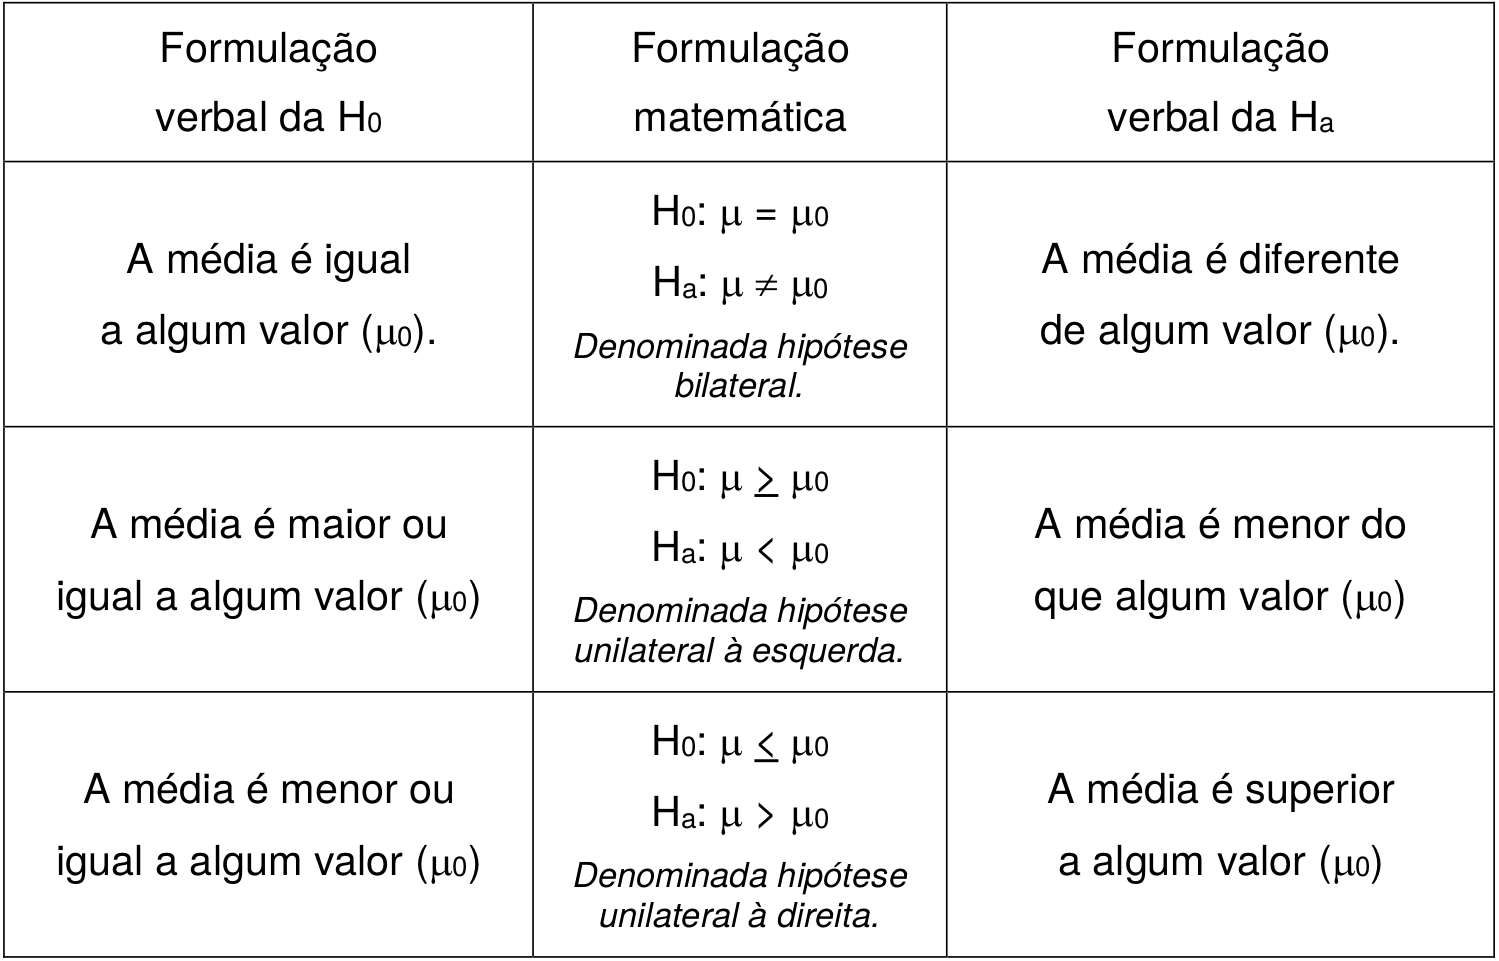
\includegraphics[scale=1.2]{testes-hipoteses/hipoteses-estatisticas.png}
\end{figure}

\section{Tipos de Erro e Nível de Significância}

Não importando qual das hipóteses representa a alegação, você começará sempre um teste de hipóteses assumindo que a condição de igualdade na hipótese nula é verdadeira. Assim, quando realizar um teste de hipóteses, você deve tomar uma de duas decisões: rejeitar a hipótese nula ou aceitar a hipótese nula.

Uma vez que sua decisão baseia-se em informação incompleta (uma amostra em vez de toda a população), há sempre a possibilidade de se tomar a decisão errada. A figura \ref{fig:resultados-teste-hipoteses} mostra os quatro resultados possíveis de um teste de hipóteses.

\begin{figure}[h]
	\center
	\caption{Possíveis Resultados para um Teste de Hipóteses}	
	\label{fig:resultados-teste-hipoteses}
	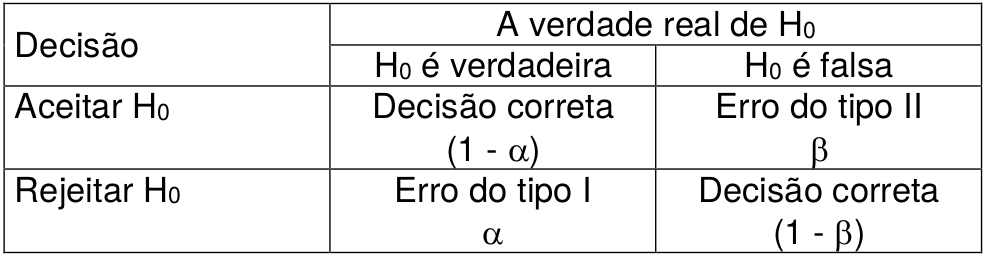
\includegraphics[scale=1.7]{testes-hipoteses/resultados-teste-hipoteses.png}
\end{figure}

O \textbf{nível de significância (\(\alpha\))} de um teste é a probabilidade de uma hipótese nula ser rejeitada, quando verdadeira. Uma das etapas de nosso processo de teste de hipóteses envolve a escolha do nível de significância. Pode-se mostrar, matematicamente, que \(\alpha\), \(\beta\) e o tamanho (n) da amostra estão todos inter-relacionados, de forma que, escolhidos quaisquer dois deles, o terceiro está
automaticamente determinado. Valem as seguintes considerações de ordem prática:
\begin{alineas}
\item Para \(\alpha\) fixo, um aumento do tamanho n da amostra ocasiona uma redução
de \(\beta\); isto é, uma amostra maior reduz a chance de cometermos o erro de aceitar a hipótese nula quando ela é falsa.
\item Para um tamanho n, fixo, de amostra, uma diminuição de \(\alpha\) acarreta um aumento de \(\beta\); reciprocamente, um aumento de \(\alpha\) acarreta uma diminuição de \(\beta\).
\item Para reduzir \(\alpha\) e \(\beta\), devemos aumentar o tamanho da amostra.
\end{alineas}

\section{Estatística de Teste, Região Crítica e Valor Crítico}

A \textbf{estatística de teste} é uma estatística amostral, ou um valor baseado nos dados
amostrais. Utiliza-se uma estatística de teste para tomar uma decisão sobre a rejeição ou não da hipótese nula. A \textbf{região crítica} é o conjunto de todos os valores da estatística de teste que levam à rejeição da hipótese nula. O \textbf{valor crítico} é o valor, ou valores, que separa(m) a região crítica dos valores da estatística de teste que não levam à rejeição da hipótese nula. Os valores críticos dependem da natureza da hipótese nula, da distribuição amostral principal, e do nível de significância.

O método clássico de testes de hipóteses  utilizando região crítica constiste nos seguintes passos:
\begin{alineas}
\item Identificar a hipótese nula (contém a condição de igualdade) e a hipótese alternativa (complementar);
\item Escolher o nível de significância com base na gravidade do erro tipo I. São
muito comuns os valores 0,05 e 0,01;
\item Identificar o teste a ser utilizado;
\item Determinar a estatística de teste;
\item Determinar o(s) valor(es) crítico(s) e a região crítica;
\item Rejeitar \(H_0\) se a estatística de teste está na região crítica. Aceitar \(H_0\) se a estatística de teste não está na região crítica;
\item Formular uma conclusão que descreva a conseqüência prática dos dados e dos cálculos.
\end{alineas}

\section{Teste z para uma Amostra (\(\sigma\) conhecido)}

O teste z é utilizado em testes de hipóteses para a média quando valor do desvio padrão (\(\sigma\) é conhecido. Identificadas as hipóteses estatísticas (\(H_0\) e \(H_a\)) e definido o nível de significância (\(\alpha\)), podemos proceder ao cálculo da estatística de teste utilizando a fórmula a seguir.

\[\beq{ z_{teste} = \frac{\hat{x}-\mu_0}{\frac{\sigma}{\sqrt{n}}} } \]

Onde \(\mu_0\) representa o valor da média que está sendo testado, \(\sigma\) representa o desvio padrão populacional, n é o tamanho da amostra e \(\hat{x}\) é a média da amostra.

\subsection{Com base no nível de significância (\(\alpha\))}

\begin{itemize}
	\item Fornecidos: \(\alpha\), \(\mu_0\), \(\hat{x}\) e \(\sigma\)
	\item Aplicar a fórmula de \(z_{teste}\)
	\item Encontrar \(z_{\alpha}\) considerando:
	\begin{itemize}
		\item O sinal de \(z_{teste}\)
		\item O tipo de hipótese (unilateral à esquerda, à direita ou bilateral)
		\item A interpretação da probabilidade na Tabela da Normal Reduzida
	\end{itemize}
\end{itemize}		
	
\subsection{Com base no valor \(p\)}

\begin{itemize}
	\item Fornecidos: \(\alpha\), \(\mu_0\), \(\hat{x}\) e \(\sigma\)
	\item Aplicar a fórmula de \(z_{teste}\)
	\item Encontrar \(p\) considerando:
	\begin{itemize}
		\item O sinal de \(z_{teste}\)
		\item O tipo de hipótese: unilateral à esquerda, à direita ou bilateral 
		\item \(p\) acompanha \(H_a\)
		\item A interpretação da probabilidade na Tabela da Normal Reduzida
		\item Interpretação: comparar \(p\) e \(\alpha\). Se \(p \leq \alpha\) a hipótese nula deve ser rejeitada.
	\end{itemize}
\end{itemize}		

\subsection{Com base no intervalo de confiança}

A correspondência direta entre um intervalo de confiança e um teste de hipótese pode ser feita somente quando o teste é bilateral.

\section{Teste t para uma amostra (\(\sigma\) desconhecido)}

O teste t é utilizado em testes de hipóteses para a média quando valor do desvio padrão (\(\sigma\) é desconhecido. Nesse caso, deve utilizar o desvio padrão amostral (\(s\)) e a distribuição t-Student. Identificadas as hipóteses estatísticas (\(H_0\) e \(H_a\)) e definido o nível de significância (\(\alpha\)), podemos proceder ao cálculo da estatística de teste utilizando a fórmula a seguir.

\[\beq{ t_{teste} = \frac{\hat{x}-\mu_0}{\frac{s}{\sqrt{n}}} } \]

Onde \(\mu_0\) representa o valor da média que está sendo testado, \(s\) representa o desvio padrão amostral, n é o tamanho da amostra e \(\hat{x}\) é a média da amostra.

O valor crítico é obtido na tabela t-Student, a partir do número de graus de liberdade (n -1). Após determinar o número de graus de liberdade (na linha da tabela) e localizar, na coluna, o valor correspondente à área da cauda que se deseja obter, o valor crítico será o valor que corresponde ao cruzamento da linha e da coluna que foram determinados. Lembrando que se um valor crítico está localizado na cauda esquerda, devemos considerá-lo negativo.

\subsection{Com base no valor \(p\)}

\begin{itemize}
	\item Fornecidos: \(\alpha\)\footnote{Lembrar de que \(\alpha\) é uma probabilidade.}, \(\mu_0\), \(\hat{x}\) e \(s\)
	\item Aplicar a fórmula para encontrar o \(t_{teste}\)
	\item Encontrar \(p\) considerando:
	\begin{itemize}
		\item O sinal de \(t_{teste}\)
		\item O tipo de hipótese (unilateral à esquerda, à direita ou bilateral)
		\item A interpretação da probabilidade na Tabela da t-Student:
			\begin{itemize}
				\item Buscar o valor mais próximo do \(t_{teste}\) na linha do grau de liberdade
				\item O valor de \(p\) é o cabeçalho correspondente ao valor encontrado na tabela t-Student
			\end{itemize}
		\item Interpretação: comparar \(p\) e \(\alpha\). Se \(p \leq \alpha\) a hipótese nula deve ser rejeitada.
	\end{itemize}
\end{itemize}

\subsection{Com base no intervalo de confiança}

A correspondência direta entre um intervalo de confiança e um teste de hipótese pode ser feita somente quando o teste é bilateral.

\section{Teste de Hipóteses para a Proporção}

Os testes de hipóteses para proporções são adequados quando os dados sob análise consistem de contagens ou frequências de itens. A finalidade de tais testes é avaliar afirmações sobre a proporção (ou percentagem) de uma população.

Suposições:
\begin{itemize}
	\item Condições para um experimento binomial
	\item Condições \(n.p_0\geq5\) e \(n.(1-p_0)\geq5\)
\end{itemize}

Estatística de teste:

 \[\beq{ z_{teste} = \frac{\hat{p}-p_0}{\sqrt{\frac{p_0(1-p_0)}{n}}} }\]
 
Em muitos aspectos, o teste de hipóteses para uma proporção se assemelha grandemente ao teste z, principalmente pelo fato de que utilizam a mesma distribuição de probabilidades. Dessa forma, a região crítica, o valor crítico e o valor p para o teste de proporção são obtidos exatamente da mesma maneira que o teste z para uma média.

\section{Teste z para Comparação de Duas Proporções}

Um teste z de duas amostras é usado para testar a diferença entre duas proporções \(p_1\) e \(p_2\) quando uma amostra é selecionada aleatoriamente de cada população.

Condições:
\begin{itemize}
	\item As amostras devem ser selecionadas aleatoriamente.
	\item As amostras devem ser independentes.
	\item As amostras devem ser grandes o suficiente para usar uma distribuição normal de amostragem (\( n_1p_1 > 5, n_1q_1 > 5, n_2p_2 > 5 \) e \( n_2q_2 > 5. \)).
\end{itemize}

Notação:
\begin{itemize}
	\item \(n_1 = \) tamanho da 1\textsuperscript{a} amostra
	\item \(n_2 = \) tamanho da 2\textsuperscript{a} amostra
	\item \(x_1 = \) número de sucessos da 1\textsuperscript{a} amostra	
	\item \(x_2 = \) número de sucessos da 2\textsuperscript{a} amostra		
	\item \(\hat{p}_1 = \) proporção de sucessos da 1\textsuperscript{a} amostra	
	\item \(\hat{p}_2 = \) proporção de sucessos da 2\textsuperscript{a} amostra		
\end{itemize}

\subsection{Abordagem pelo valor p}

\begin{verbatim}
	Estratégia sugerida: Geogebra 
\end{verbatim}

Estatística de teste:

\[\beq{ z = \frac{\hat{p_1}-\hat{p_2}}{\sqrt{\frac{\bar{p}(1-\bar{p})}{n_1}+\frac{\bar{p}(1-\bar{p})}{n_2}} }}\]

onde, a estimativa ponderada para \(p_1\) e \(p_2\) pode ser obtida por:

\[\bar{p}=\frac{n_1\hat{p}_1 + n_2\hat{p}_2}{n_1+n_2}\]

Conclusão:
\begin{itemize}
	\item Se \(p \leq \alpha\), rejeitarmos \(H_0\).
	\item Se \(p > \alpha\), aceitarmos \(H_0\).
\end{itemize}

\subsection{Abordagem pelo intervalo de confiança}

\begin{verbatim}
	Estratégia sugerida: Python 
\end{verbatim}

\[\beq{ (\hat{p}_1-\hat{p}_2) \pm z_{\frac{1-\alpha}{2}} \sqrt{\frac{\bar{p}(1-\bar{p})}{n_1}+\frac{\bar{p}(1-\bar{p})}{n_2}} }\]

Interpretação:

\begin{itemize}
	\item se o intervalo contém 0 (zero) há indícios de que as duas proporções são iguais, caso contrário, se o intervalo não contém 0 (zero) pode-se concluir com \( 100(1-\alpha)\% \) de confiança que as duas proporções são diferentes.
		\item Se os limites do intervalo do confiança apresentam sinal negativo (-) pode-se dizer que a proporção da 2\textsuperscript{a} amostra é maior do que a proporção da 1\textsuperscript{a} amostra.
	\item Ao contrário, se os limites do intervalo apresentarem sinal positivo (+) conclui-se que a proporção da 1\textsuperscript{a} amostra é maior que a proporção da 2\textsuperscript{a} amostra.
\end{itemize}

\section{Teste t para Comparação de Duas Médias (Amostras Pareadas)}

Uma amostra pareada corresponde ao levantamento de dados da mesma amostra em duas situações nas quais tenha interferido algum fator cujo efeito deseja-se avaliar (Ex.: Comparar o peso de um grupo de pessoas antes e depois de passarem por uma dieta rigorosa).

Suposições:
\begin{itemize}
	\item Deve-se escolher de maneira aleatória duas amostras dependentes de duas populações.
	\item Ambas as populações devem ter distribuição Normal. Se elas se afastam radicalmente da distribuição Normal, devemos utilizar os métodos não-paramétricos.
\end{itemize}

\subsection{Abordagem pelo valor p}

\begin{verbatim}
	Estratégia sugerida: Python 
\end{verbatim}

\begin{alineas}
	\item Estabeleça o nível de significância (\(\alpha\)) a ser adotado. Se \(\alpha\) não for fornecido, adotar o valor padrão 0.05.
	\item Estabelecer as hipóteses:
		\begin{alineas}
			\item \(H_0\): Médias pareadas iguais (antes e depois): \(\mu_1 = \mu_2\)
			\item \(H_1\): Médias pareadas significativamente diferentes\footnote{Nesse material, trataremos somente a hipótese bilateral.}: \(\mu_1 \neq \mu_2\)
		\end{alineas}
	\item Encontrar o valor \(\bar{d}\) que é a média das diferenças \(d_i\): 

	\[\beq{ \bar{d} = \frac{\sum{d_i}}{n} }\]

	\item Calcular o desvio padrão \(s_d\) das diferenças \(d_i\):

	\[\beq{ s_d = \sqrt{\frac{n(\sum{d_i^2})(\sum{d_i})^2}{n(n-1)}} }\]	
	
	\item Calcular a estatística de teste \(T_p\):
	
	\[\beq{ T_p = \frac{\bar{d}}{ \frac{s_d}{\sqrt{n}}} }\]
	
	\item Calcular o valor \textbf{p}: \(p = 2 \times P(t>|T_p|) \), com n-1 graus de liberdade.

	\item Conclusão:
		\begin{alineas}
			\item Se p \(\leq\) nível de significância (\(\alpha\)), então há indícios para rejeitarmos \(H_0\).
			\item Se p > nível de significância (\(\alpha\)), então há evidências suficientes para aceitarmos \(H_0\).
		\end{alineas}

\subsection{Abordagem pelo intervalo de confiança}

\begin{verbatim}
	Estratégia sugerida: Python 
\end{verbatim}

\[\beq{ \bar{d} \pm t_{n-1;\frac{\alpha}{2}} \times \frac{s_d}{\sqrt{n}}  }\]
	
\end{alineas}

\section{Teste F para Comparação de Duas Variâncias (Bilateral)}

\begin{verbatim}
	Estratégia sugerida: Python 
\end{verbatim}

Esse teste é, muitas vezes, usado em conexão com o teste t-Sudent para duas médias (amostras
independentes), em que é necessário verificar a homocedasticidade (igualdade) ou
heterocedasticidade (diferença) das variâncias. Para duas amostras aleatórias e independentes, de tamanhos \(n_1\) e \(n_2\), retiradas de duas populações normais com variâncias \(\sigma_1^2\) e
\(\sigma_2^2\). Desejamos testar a hipótese bilateral: 

\[H_0: \sigma_1^2 = \sigma_2^2\]

\[H_a: \sigma_1^2 \neq \sigma_2^2\]

Estatística de teste:

\[ F = \frac{\sigma_1^2}{\sigma_2^2} \]

Valores críticos:

\[\beq{ F_L = \frac{1}{F_{n_2-1;n1-1;\frac{\alpha}{2}}} }\]

\[\beq{ F_R = F_{n_1-1;n2-1;\frac{\alpha}{2}} }\]

Os valores \( F_{n_2-1;n1-1;\frac{\alpha}{2}} \) e \(F_{n_1-1;n2-1;\frac{\alpha}{2}}\) são encontrados na  tabela F. Para um nível de significância \(\alpha\):
\begin{itemize}
	\item Rejeitar \(H_0\) se \(F < F_L\) ou se \(F>F_R\)
	\item Caso contrário, não rejeitamos \(H_0\)
\end{itemize}

\section{Teste t para Comparação de Duas Médias (Amostras Independentes)}

\begin{verbatim}
	Estratégia sugerida: Python
\end{verbatim}

O teste t-Student, ou simplesmente teste t, é o método mais utilizado para se avaliarem as diferenças entre as médias de dois grupos para os casos em que as variâncias populacionais são desconhecidas.


Suposições:
\begin{itemize}
	\item As duas amostras são independentes;
	\item As duas amostras são extraídas aleatoriamente de populações distribuídas normalmente.
	\item Caso a suposição de normalidade não seja comprovada, pode-se optar por realizar testes não-paramétricos. Estes não necessitam de pressupostos sobre a distribuição dos dados.
\end{itemize}

Consideramos dois casos distintos para o teste de hipóteses para comparação de duas médias. O primeiro caso em que as variâncias das populações são desconhecidas, porém iguais (homocedasticidade) e o segundo caso em que as variâncias são desconhecidas e distintas (heterocedasticidade).

\subsection{As duas populações parecem ter variâncias iguais (Homocedásticas)}

Notação:
\begin{itemize}
	\item \(x_1\) = média da 1\textsuperscript{a} amostra
	\item \(x_2\) = média da 2\textsuperscript{a} amostra
	\item \(n_1\) = tamanho da 1\textsuperscript{a} amostra
	\item \(n_2\) = tamanho da 2\textsuperscript{a} amostra
	\item \(s_1^2\) = variância da 1\textsuperscript{a} amostra
	\item \(s_2^2\) = variância da 2\textsuperscript{a} amostra 
\end{itemize}


Estatística de Teste:

\[\beq{ t_0 = \frac{(\bar{x}_1-\bar{x}_2)}{\sqrt{\frac{s_{comb}^2}{n_1} + \frac{s_{comb}^2}{n_2}}} }\]

A variância combinada \(s_{comb}^2\) calculada a partir da seguinte fórmula:

\[\beq{ s_{comb}^2 = \frac{(n_1-1)s_1^2 + (n_2-1)s_2^2}{(n_1-1)+(n_2-1)}  }\]

Número de graus de liberdade quando as variâncias amostrais são combinadas: \( g.l. = n_1 + n_2 - 2 \)

Conclusão:
\begin{itemize}
	\item Se \(p \leq \alpha\), rejeitarmos \(H_0\).
	\item Se \(p > \alpha\), aceitamos \(H_0\).
\end{itemize}

Pelo intervalo de confiança:

\[\beq{ (\bar{x}_1 - \bar{x}_2) \pm t_{gl;\frac{\alpha}{2}}\sqrt{\frac{s_{comb}^2}{n_1} + \frac{s_{comb}^2}{n_2}} }\]

Interpretação:

\begin{itemize}
	\item se o intervalo contém 0 (zero) há indícios de que as duas médias são iguais, caso contrário, se o intervalo não contém 0 (zero) pode-se concluir com \( 100(1-\alpha)\% \) de confiança que as duas médias são diferentes.
		\item Se os limites do intervalo do confiança apresentam sinal negativo (-) pode-se dizer que a média da 2\textsuperscript{a} amostra é maior do que a média da 1\textsuperscript{a} amostra.
	\item Ao contrário, se os limites do intervalo apresentarem sinal positivo (+) conclui-se que a média da 1\textsuperscript{a} amostra é maior que a média da 2\textsuperscript{a} amostra.
\end{itemize}

\subsection{As duas populações parecem ter variâncias desiguais (Heterocedásticas)}

Notação:
\begin{itemize}
	\item \(x_1\) = média da 1\textsuperscript{a} amostra
	\item \(x_2\) = média da 2\textsuperscript{a} amostra
	\item \(n_1\) = tamanho da 1\textsuperscript{a} amostra
	\item \(n_2\) = tamanho da 2\textsuperscript{a} amostra
	\item \(s_1^2\) = variância da 1\textsuperscript{a} amostra
	\item \(s_2^2\) = variância da 2\textsuperscript{a} amostra 
\end{itemize}

Estatística de teste:

\[\beq{ t_0 = \frac{(\bar{x}_1-\bar{x}_2)}{\sqrt{\frac{s_1^2}{n_1} + \frac{s_2^2}{n_2}}} }\]

Número de graus de liberdade (\( g.l.) \) é o menor dos dois: \(n_1 - 1\)  ou  \(n_2 - 1\)

Intervalo de confiança (para hipóteses bilaterais): 

\[\beq{ (\bar{x}_1 - \bar{x}_2) \pm t_{gl;\frac{\alpha}{2}}\sqrt{\frac{s_1^2}{n_1} + \frac{s_2^2}{n_2}} }\]

A conclusão do teste de hipóteses utilizando o valor p ou o intervalo de confiança deve ser feita da mesma maneira que no caso das homocedásticas.

\begin{apendicesenv}
\chapter{Tabela de Probabilidades - Distribuição Normal Padrão}

\begin{figure}[h]
	\center
	\label{fig:tab-prob-normal-padrao}
	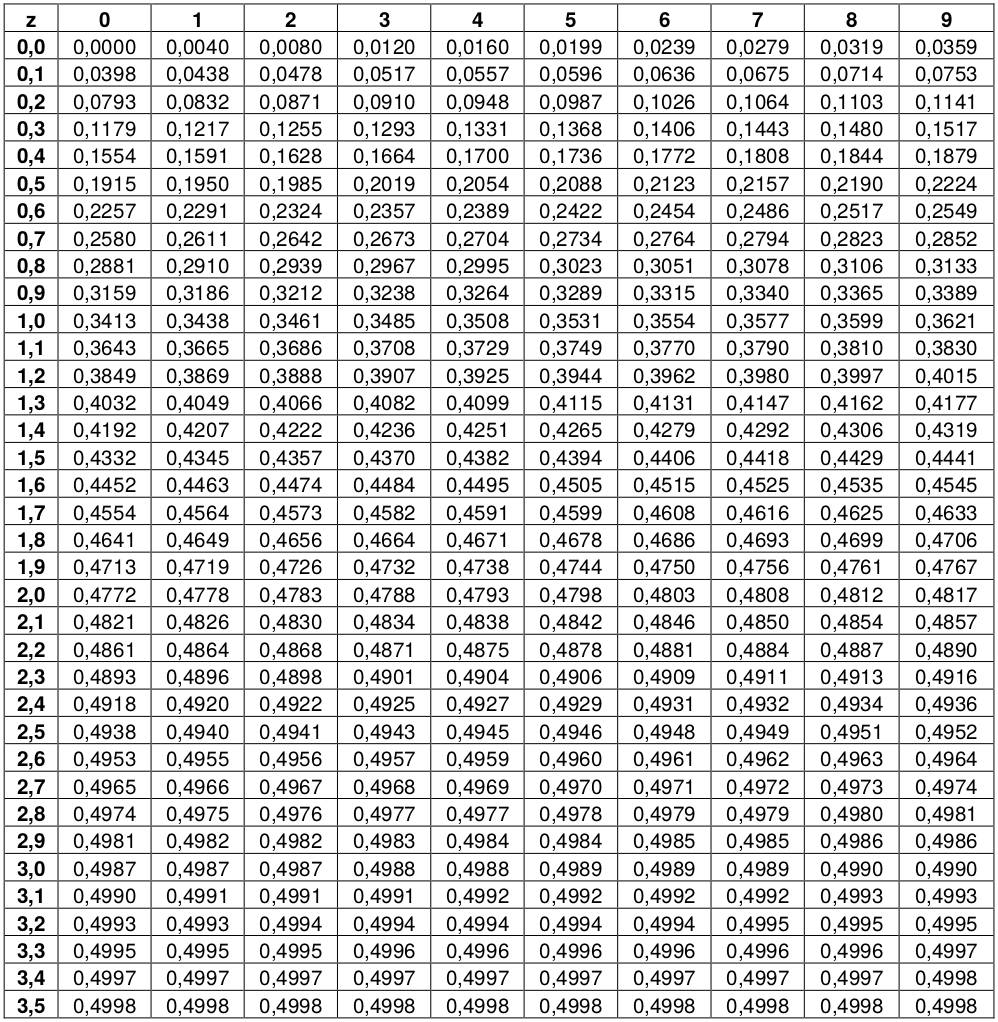
\includegraphics[scale=2]{apendices/prob-normal-padrao.png}
\end{figure}

Onde:
\begin{itemize}
	\item O valores de \(z\) estão nos cabeçalhos de linha e coluna;
	\item As probabilidades estão no centro.
\end{itemize}


\chapter{Tabela de Probabilidades - Distribuição t-Student}

\begin{figure}[h]
	\center
	\label{fig:tab-prob-t-student}
	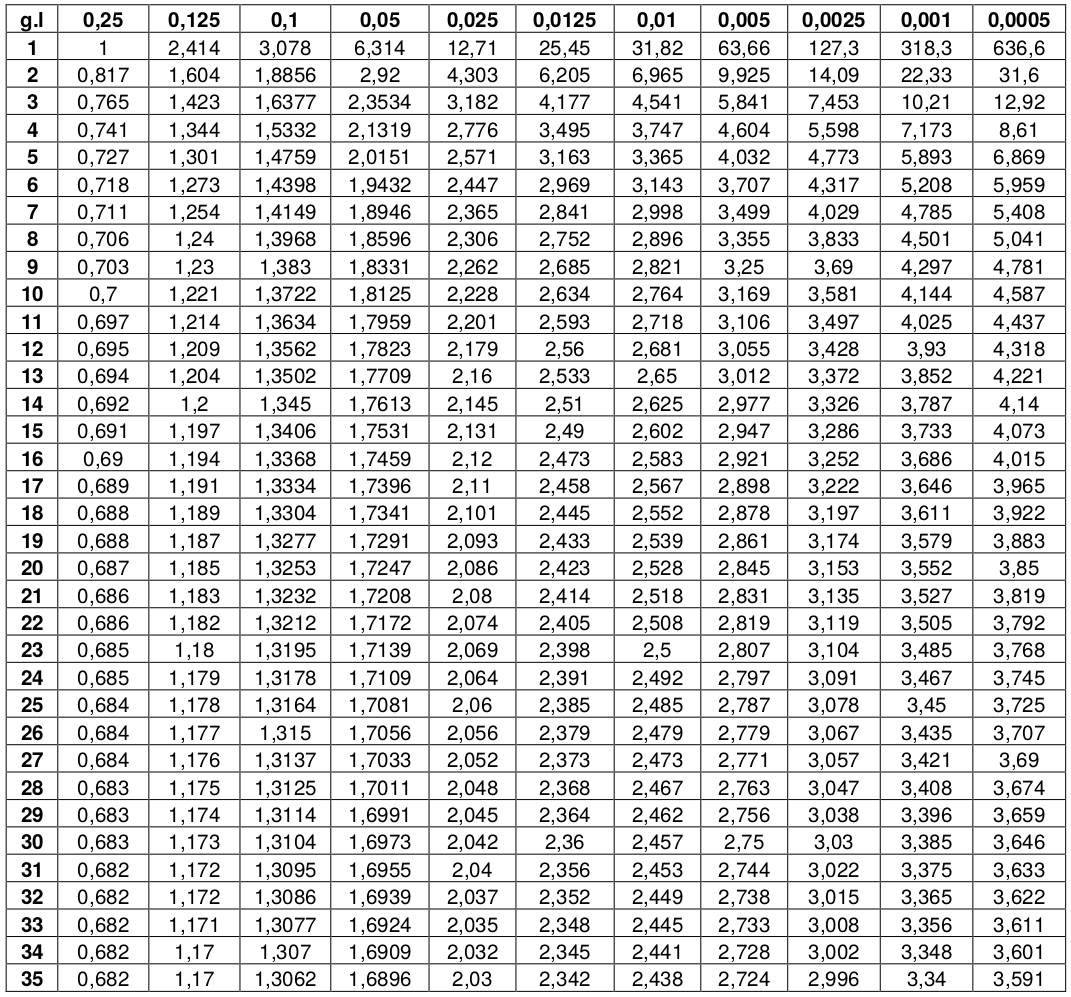
\includegraphics[scale=1.85]{apendices/prob-t-studend.png}
\end{figure}
\end{apendicesenv}

\end{document}